\chapter{Použité technologie}
\label{3-technologie}

Třetí kapitola stručně představuje jednotlivé technologie použité při
tvorbě webového administrátorského rozhraní.

\section{LDAP}
% https://en.wikipedia.org/wiki/Lightweight_Directory_Access_Protocol

Lightweight Directory Access Protocol neboli \zk{LDAP} je otevřený, standardizovaný protokol. Slouží k přístupu k datům, jejich úpravám a ukládání na adresářovém serveru přes Internet Protocol (\zk{IP}). Je vhodný pro správu informací o uživatelích. Je nezávislý na operačním systému.

Protokol LDAP vychází ze standardu X.500, jehož je odlehčenou variantou. Někdy je nazýván X.500-lite.\footnote{https://www.webopedia.com/TERM/L/LDAP.html}

\subsection{OpenLDAP}

% neznam licenci
\begin{figure}[H] \centering
      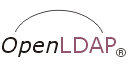
\includegraphics[width=100pt]{./pictures/LDAPlogo.png}
      \caption[OpenLDAP logo]{OpenLDAP logo (zdroj:
\href{http://www.openldap.org/images/headers/LDAPlogo.gif}{OpenLDAP.org})}
      \label{fig:ldap}
  \end{figure}

OpenLDAP je otevřená (open-source) implementace protokolu \zk{LDAP}.

\subsection{django-python3-ldap}
https://github.com/etianen/django-python3-ldap/blob/master/README.rst

\subsection{ldap3}
https://ldap3.readthedocs.io/welcome.html


\newpage

\section{Python}

\begin{figure}[H] \centering
      
\includegraphics[width=150pt]{./pictures/python-logo-master-v3-TM.png}
      \caption[Python logo]{Python logo (zdroj:
\href{https://www.python.org/static/community_logos/python-logo-master-v3-TM.png}{Python.org})}
      \label{fig:python}
  \end{figure}
  
Python je vysokoúrovňový, interpretovaný programovací jazyk. Podporuje
procedurálně i objektově orientované programování, je výkonný, zároveň
má velmi jednoduchou a čistou syntax. V ostatních jazycích je
odsazování řádků doporučeno z hlediska přehlednosti, u Pythonu je
základním stavebním kamenem a je povinné.

Guido van Rossum, autor první verze Pythonu vydané v roce 1991, se
rozhodl vyřešit nedostatečnost jazyků, které byly používány v jeho
zaměstnání, a napsat jazyk splňující jeho potřeby. Při vývoji se
inspiroval především v jazycích ABC a~Modula-3. Jednou ze snah bylo
vytvoření jazyka otevřeného dalším rozšířením a~propojením s jinými
jazyky (např. C++). Dnes je Python vyvíjen jako open source projekt
pod záštitou neziskové organizace Python Software Foundation
(\zk{PSF}). Je distribuován pod licencí \zk{PSF}, která je
kompatibilní s \zk{GPL}. Je možné ho nainstalovat na běžné platformy
jako Windows, Unix nebo Mac OS, pro Linux je většinou součástí
základní instalace. Při vyvarování se systémově závislých funkcí je
přenositelný mezi~platformami bez jakýchkoli změn.

Python má široké využití, od jednoduchých programů po rozsáhlé
aplikace. Právě pro tyto možnosti, univerzálnost, přehlednost kódu a
výkonnost z něj udělaly programovací jazyk, který je mezi začátečníky ve
velké oblibě. Během krátké doby v~něm funkční skript zvládne napsat
každý.
  
% (3) https://docs.python.org/3/faq/general.html#general-python-faq

\newpage
  
\section{Django}

\begin{figure}[H] \centering
      
\includegraphics[width=150pt]{./pictures/django-logo-positive.png}
      \caption[Django logo]{Django logo (zdroj:
\href{https://static.djangoproject.com/img/logos/django-logo-positive.png}{Djangoproject.com})}
      \label{fig:django}
  \end{figure}
  
\newpage  
  
\section{Docker}

% kouknout na licenci (můžu používat??)
\begin{figure}[H] \centering
      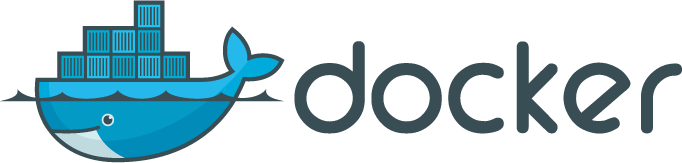
\includegraphics[width=150pt]{./pictures/Docker_(container_engine)_logo.png}
      \caption[Docker logo]{Docker logo (zdroj:
\href{https://commons.wikimedia.org/wiki/File:Docker_(container_engine)_logo.png}{Wikimedia Commons})}
      \label{fig:docker}
  \end{figure}

